\section{Additional voting behavior data}
\label{apdx:additional_results_behavior}
In this section, we describe additional voting behavior that we observed. The reason why we decided to focus on the percentage of remaining credits comes from prior literature `scarcity frames value'~\cite{Shah2015a}, a driver that makes researchers believe makes quadratic voting more accurate~\cite{chengCanShowWhat2021}. We did not follow~\citet{quarfoot2017quadratic} in counting accumulated votes over time due to varying total times across individuals.

We observed the number of vote adjustments given a remaining vote credit percentage. Figure~\ref{apdxfig:voting_all} showed all the voting actions over the remaining credit for the four experiment conditions. Here we see two distinct patterns between the short survey and the long survey in terms of participant behaviors. In long surveys, participants exhibited more actions both when the budget was abundant and when it began to run out. This pattern was more pronounced with the long two-phase interface. This difference is why we further focused on the long QS group.

\begin{figure*}[p]
    \centering
    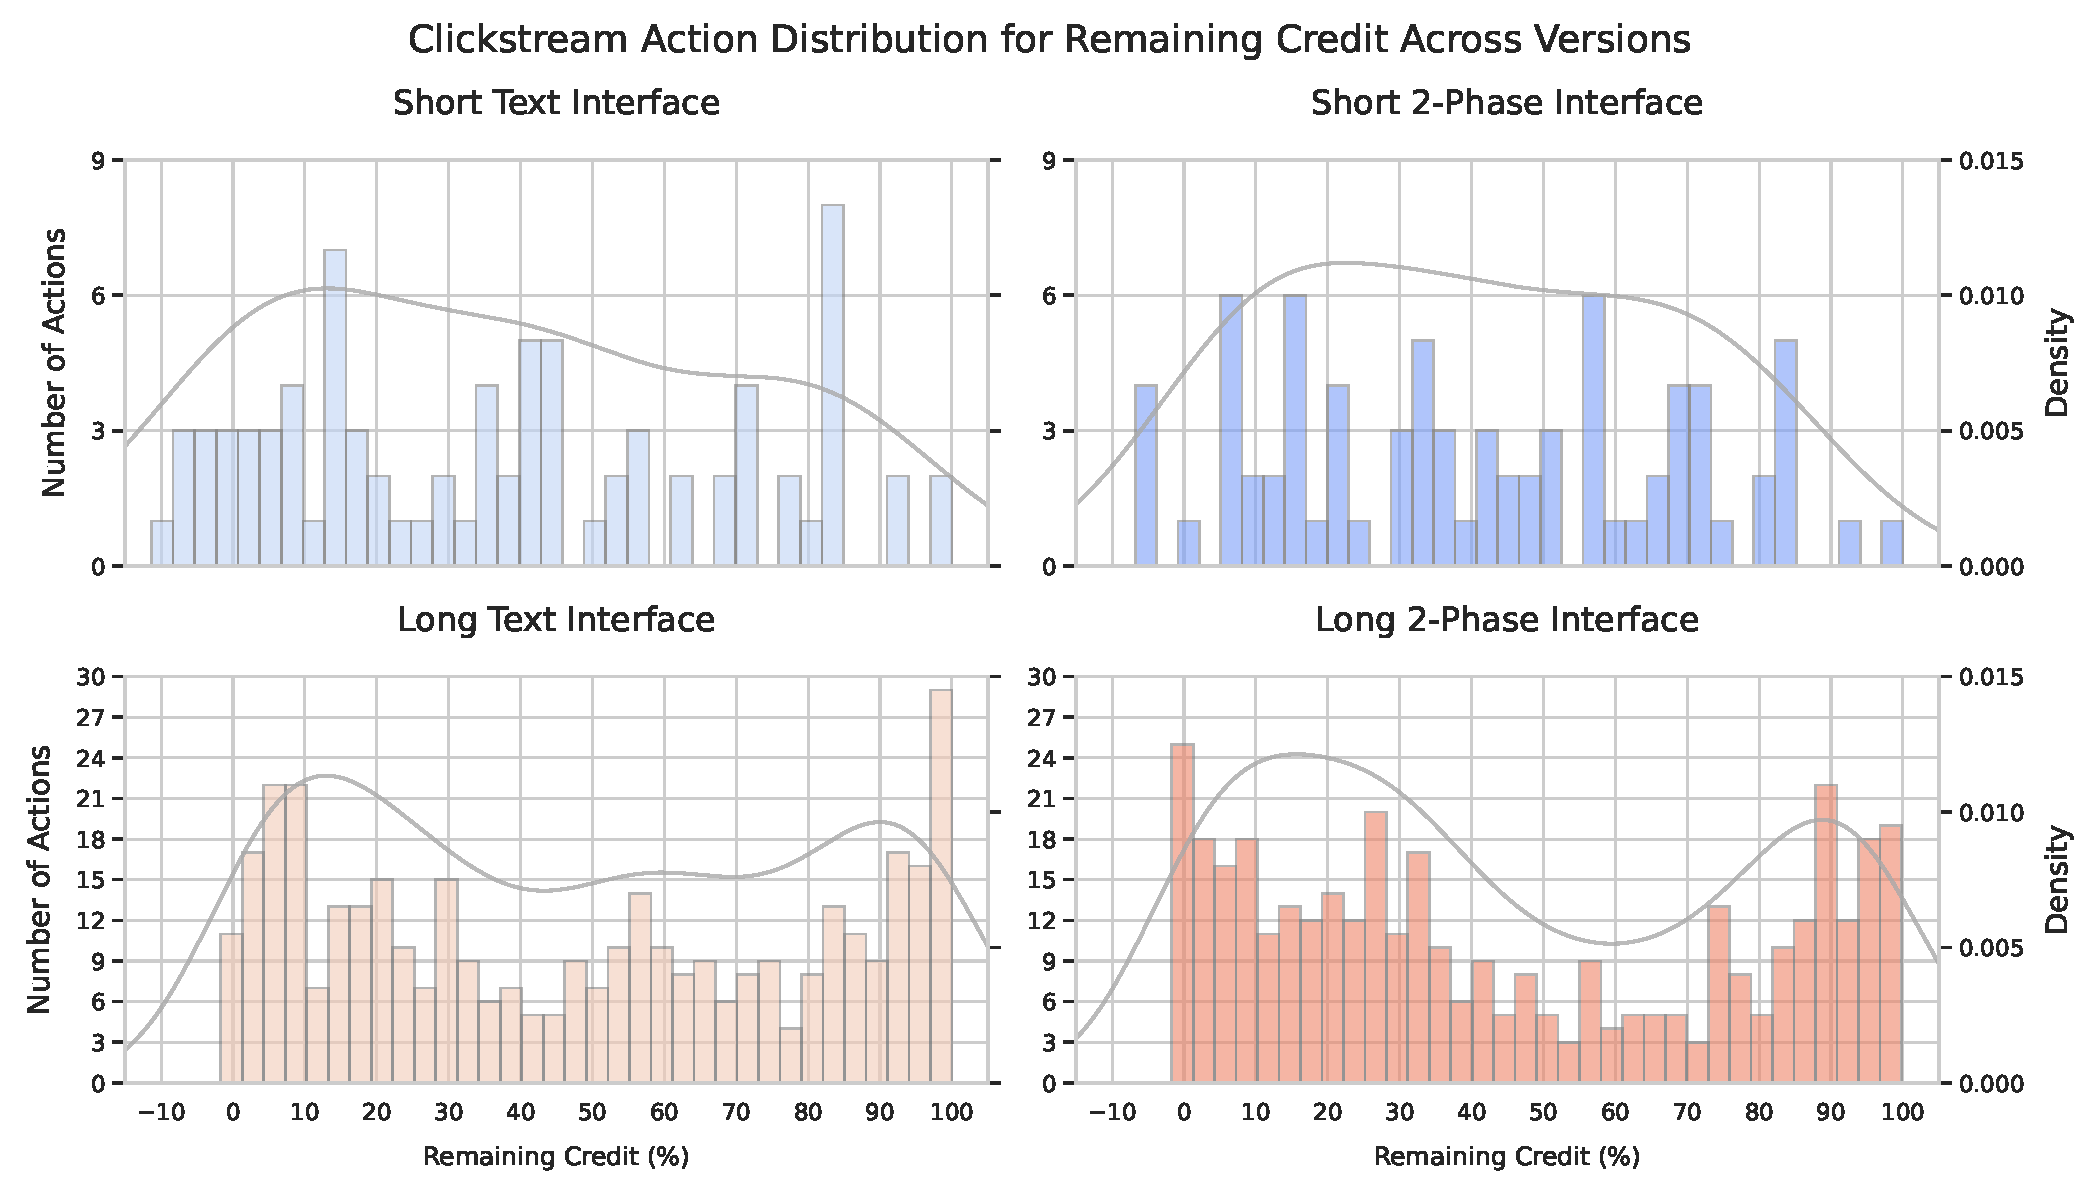
\includegraphics[width=0.9\textwidth]{content/image/results/clickstream_action_distribution.pdf}
    \caption{This plot counts the number of voting actions when there are $x$ percentages of credits remaining. A KDE plot is provided to help better understand the action distribution.}
    \Description{A four-panel histogram showing the number of voting actions across remaining credit percentages for four interface versions: Short Text, Short 2-Phase, Long Text, and Long 2-Phase. Each panel displays the number of actions on the y-axis and remaining credit on the x-axis, with an overlaid KDE curve representing density. In the top panels (Short Text and Short 2-Phase), actions are distributed relatively evenly, with small peaks around 10-20\% and 50\% remaining credit. The KDE curves show minor fluctuations. In the bottom panels (Long Text and Long 2-Phase), there are more pronounced peaks at 0-10\% and 100\% remaining credit, with broader distributions and smoother KDE curves indicating denser actions around these areas. The Long Text and Long 2-Phase interfaces exhibit more actions overall compared to the Short Text and Short 2-Phase interfaces.}
    \label{apdxfig:voting_all}
\end{figure*}

Figure~\ref{apdxfig:voting_v3_v4} presents the comparison between when participants make small or large vote adjustments at different budget levels. Revisiting the KDE curve in the second row in Figure~\ref{apdxfig:voting_all} and the curve of the second row in Figure~\ref{apdxfig:voting_v3_v4} show a stronger bimodal distribution for small vote adjustments across interfaces. In fact, the bimodal distribution is more pronounced in the two-phase interface. This suggests that participants make small adjustments both at the beginning and toward the end of the QS. However, the two-phase interface shows more frequent and faster edits towards the end. In comparison, participants also made more large vote adjustments early on that spread more equally compared to the text interface. This indicates that participants had a clearer idea of how to distribute their credits across the options.

\begin{figure*}[p]
    \centering
    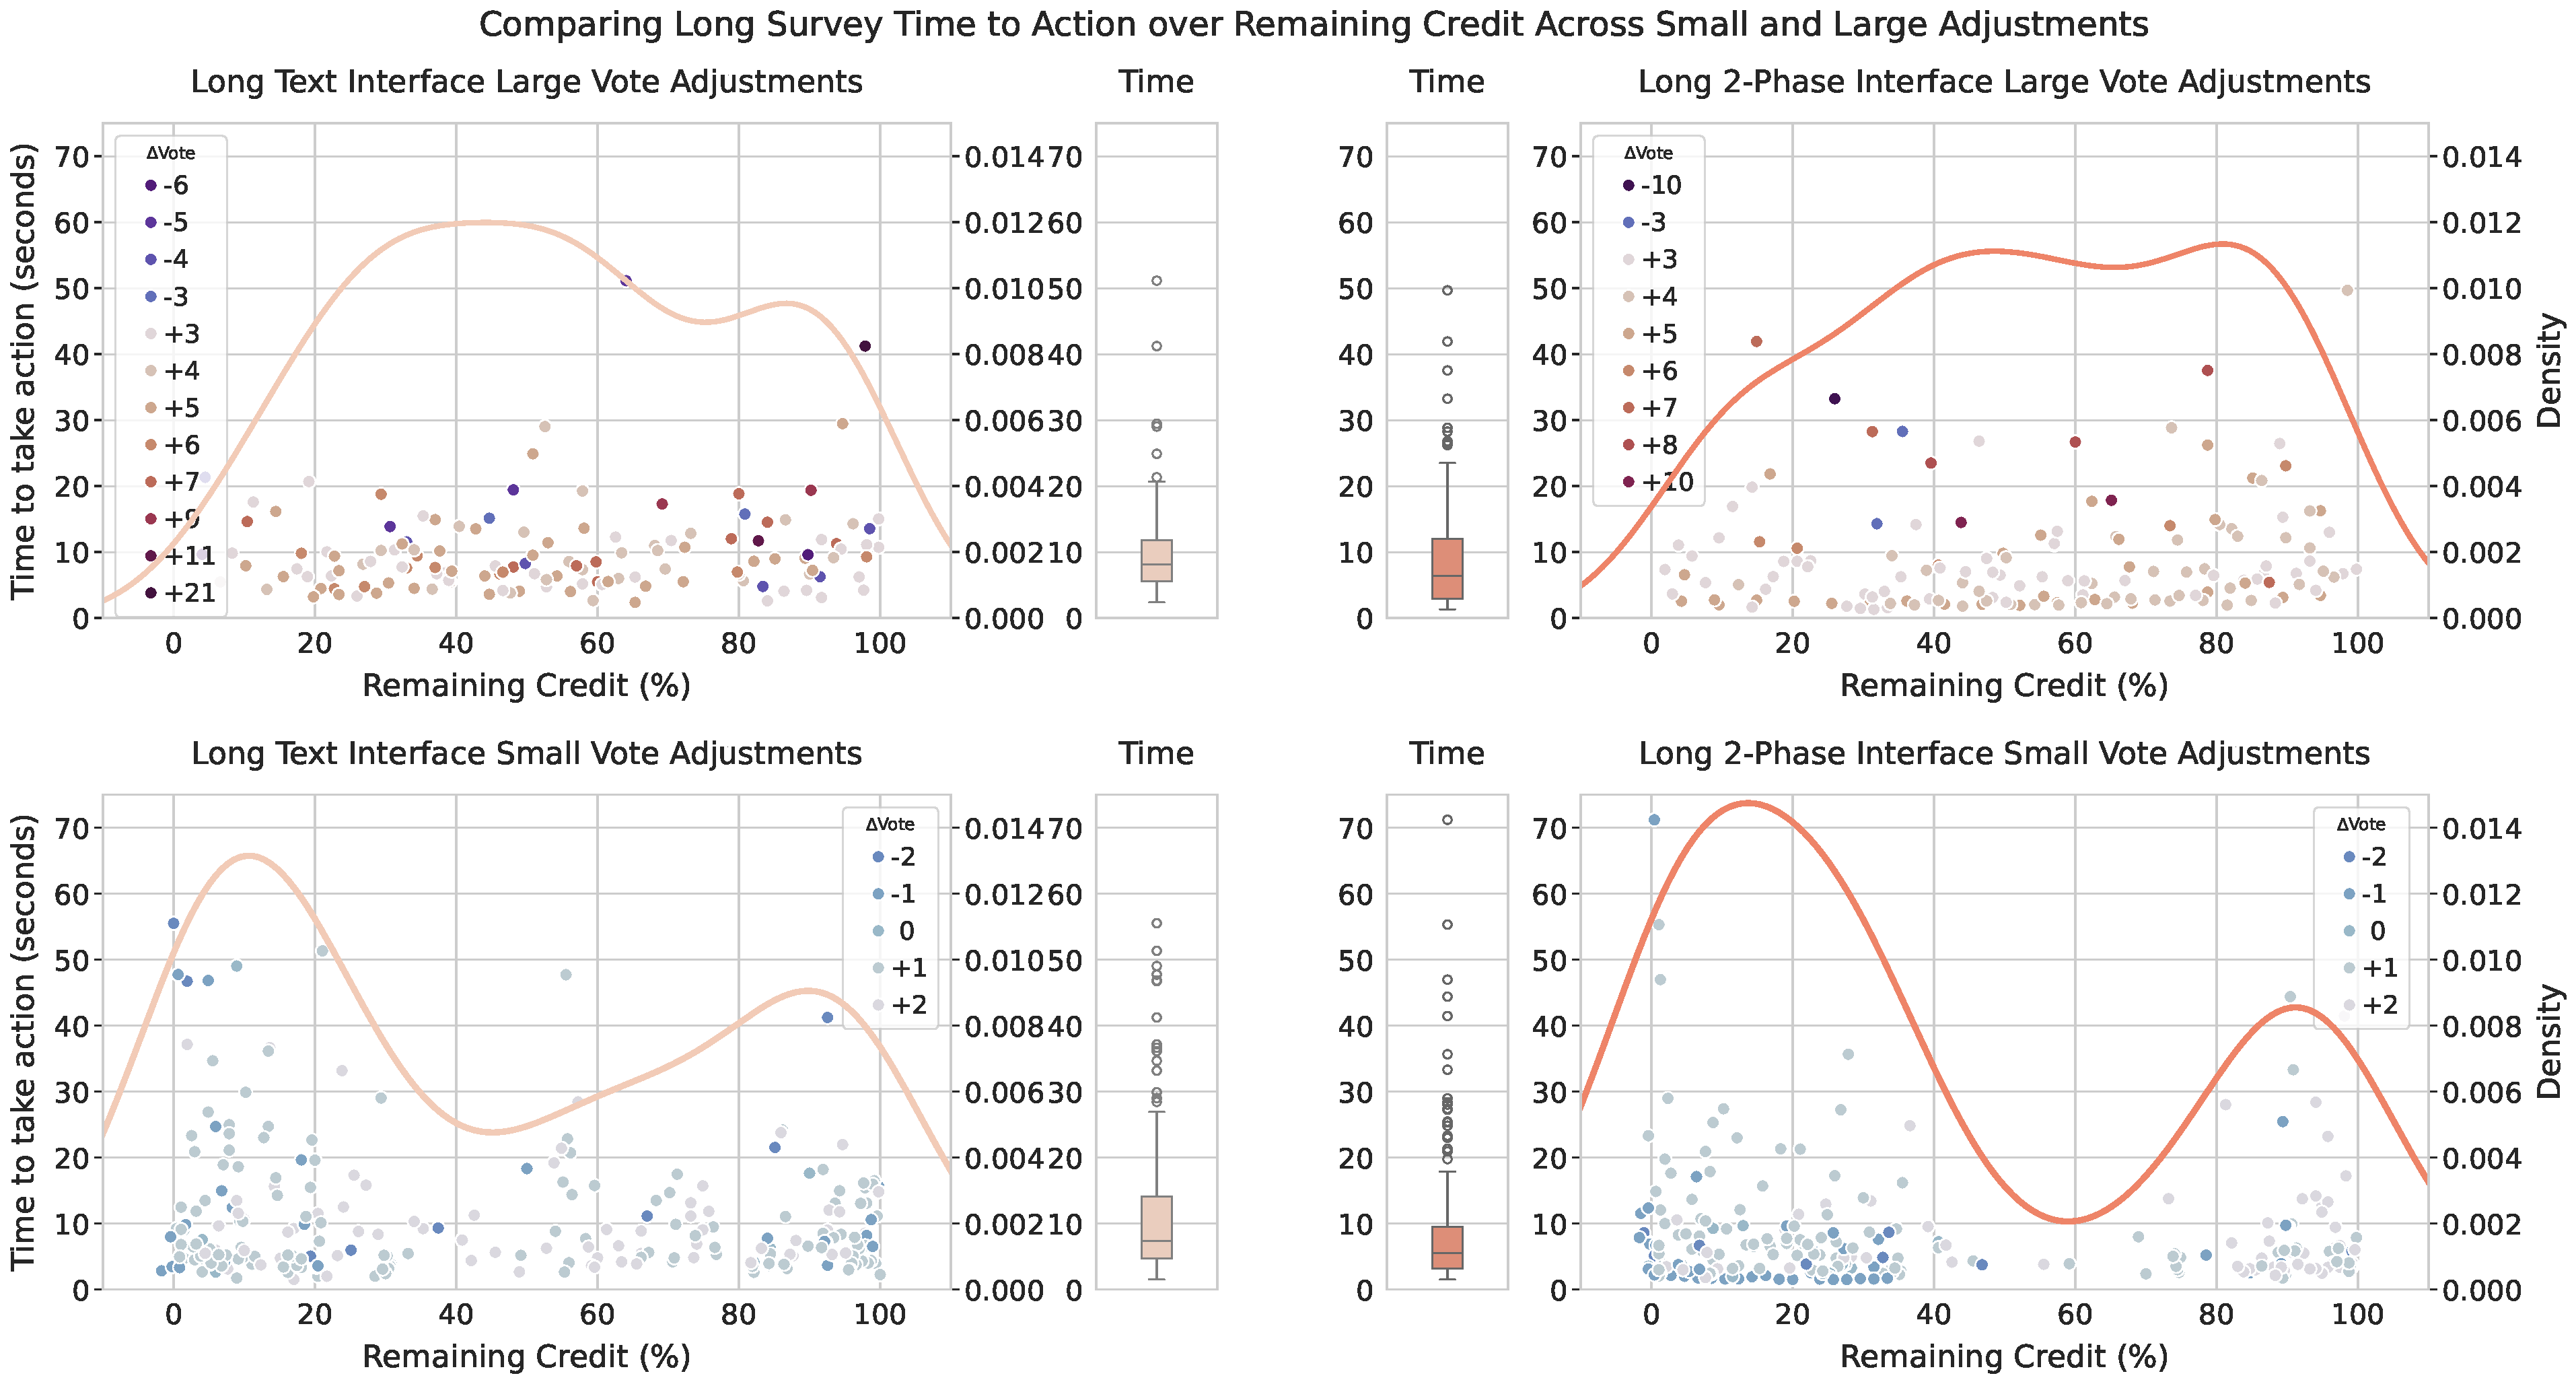
\includegraphics[width=0.9\textwidth]{content/image/results/combined_density_plots.pdf}
    \caption{This plot further separates participants' interaction behavior based on the number of votes participants adjusted. We observed a bimodal interaction pattern across long QS when small vote adjustments are made.}
    \Description{A four-panel plot comparing the time to take action in seconds over remaining credit percentages for large and small vote adjustments in the Long Text and Long 2-Phase interfaces. Each panel includes scattered points and an overlaid KDE curve. The top left panel shows large vote adjustments for the Long Text interface, with peaks in the KDE curve around 20\% and 80\% remaining credit. The top right panel shows large vote adjustments for the Long 2-Phase interface, with two peaks in the KDE curve around 10\% and 100\%. The bottom left panel shows small vote adjustments for the Long Text interface, with scattered points and peaks in the KDE curve around 10\% and 90\%. The bottom right panel shows small vote adjustments for the Long 2-Phase interface, with a KDE curve peaking around 10\% and 100\% remaining credit. Box plots on the right side of each panel summarize the distribution of time taken to adjust votes for each interface.}    
    \label{apdxfig:voting_v3_v4}
\end{figure*}

